% DO NOT COMPILE THIS FILE DIRECTLY!
% This is included by the other .tex files.

\begin{frame}[t,plain]
\titlepage
\end{frame}

% \begin{frame}{Índice}
% 	\tableofcontents
% \end{frame}

\section{Linear convection}

\begin{frame}{Linear convection problem}
	We consider the linear convection problem:
	\begin{block}{}
		\vspace*{-1cm}
		\begin{subequations}
			\label{problema:conveccion}
			\begin{align}
				\label{eq:conveccion}
				v_t+\nabla\cdot(\bbeta v)&=0&\text{in }\Omega\times(0,T),\\
				%	v &= v_{in}&\text{on }\partial\Omega_{in}\times(0,T),\\
				\label{ic:conveccion}
				v(0)&=v_0&\text{in }\Omega,
			\end{align}
		\end{subequations}
	\end{block}
	where
	\begin{itemize}
		\item $\bbeta\colon\overline{\Omega}\to\R^d$ is continuous and \alert{incompressible}, i.e, $\nabla\cdot\bbeta=0$ in $\Omega$,
		\item $\bbeta\cdot\boldsymbol{n}=0$ on $\partial\Omega$.
	\end{itemize}
	
	\vspace*{0.3cm}
	Properties:
	\begin{itemize}
		\item \alert{Existence} and \alert{uniqueness} of the solution.
		\item \alert{Mass conservation}: $\frac{d}{dt}\int_\Omega v=0$.
		\item \alert{Maximum principle}: $\min_{\overline\Omega}{v_0}\le v\le\max_{\overline\Omega}{v_0}$ in $ \overline\Omega\times (0,T)$.
	\end{itemize}
	
\end{frame}

\begin{frame}{Discontinuous Galerkin methods}
	\footnotesize
	\vspace*{-0.5cm}
	\begin{block}{}
		\begin{center}
			$\alert{\Pd_k(\T_h)}\coloneqq\left\{v_h\in L^2(\Omega)\colon v_{h|_{K_i}}\in\mathbb{P}_k(K_i)\text{ with } K_i\in\T_h,\forall i\in\left\{1,2,\ldots,N_{\T_h}\right\}\right\}$
		\end{center}
	\end{block}
	with a basis $\left\{\phi_i\right\}_{i\in\left\{1,2,\ldots,N_h \right\}}$.
	
	\vspace*{0.3cm}
	Notation:
	
	\begin{minipage}{0.69\textwidth}
	\begin{itemize}
		\item \structure{Average}: 
		$\alert{\media{v}}\coloneqq
		\begin{cases}
			\dfrac{\vK+\vL}{2}&\text{if } e=\partial K\cap\partial L\in\E_h^i\\
			\vK&\text{if }e=\partial K\in\E_h^b
		\end{cases},$
		\item \structure{Jump}: $
		\alert{\salto{v}}\coloneqq
		\begin{cases}
			\vK-\vL&\text{if } e=\partial K\cap\partial L\in\E_h^i\\
			\vK&\text{if }e=\partial K\in\E_h^b
		\end{cases},$
	\item \structure{Positive part}:
		$v_\oplus\coloneqq\displaystyle\frac{\vert v\vert +v}{2}=\max\{v,0\},$
	\item \structure{Negative part}:
	$v_{\ominus}\coloneqq\displaystyle\frac{\vert v\vert -v}{2}=-\min\{v,0\},$
	\item $
	v=v_\oplus - v_\ominus.
	$
		\end{itemize}
	\end{minipage}
	\begin{minipage}{0.29\textwidth}
		\begin{figure}
			\centering
			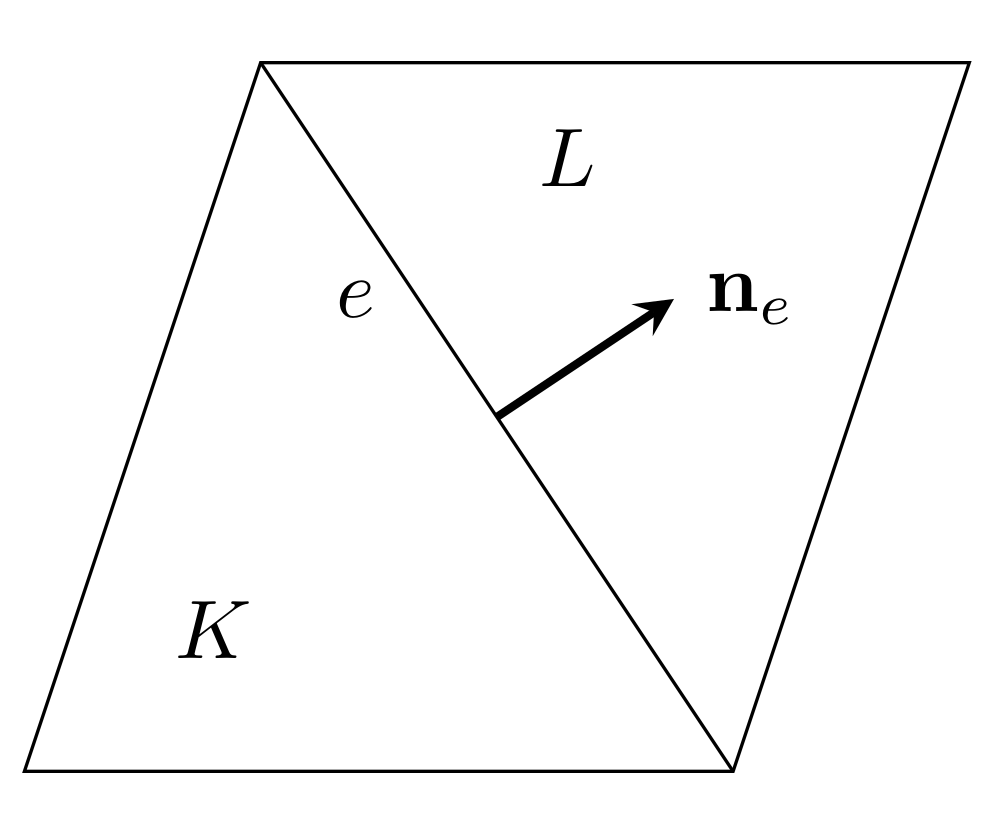
\includegraphics[scale=0.7]{img/figura_tikz.png}
			{\scriptsize\structure{Figure:} Orientation of unit normal vector.}
		\end{figure}
	\end{minipage}
\end{frame}

\begin{frame}{DG upwind method}
	\vspace*{-0.1cm}
	\begin{itemize}\itemsep1em
		\item $a_h^{\text{upw}}:\Pd_k(\T_h)\times \Pd_k(\T_h)\to\R$,
		\begin{equation*}
			\begin{aligned}
				\alert{\aupw{\bbeta}{v}{\bv}}&\coloneqq-\sum_{K\in\T_h}\int_K v (\bbeta\cdot\nabla \bv)
				\\&\quad+\sum_{e\in\E_h^i, e=K\cap L}\int_e\left( (\bbeta\cdot\nn_e)_{\oplus}\vK
				-(\bbeta\cdot\nn_e)_{\ominus} \vL\right) \salto{\bv}
			\end{aligned}
		\end{equation*}
	\end{itemize}
	
\end{frame}

\begin{frame}{Properties of the scheme for $k=0$}
	Given $v^m\in\Pd_0(\T_h)$, find $v^{m+1}\in \Pd_0(\T_h)$ such that $$\escalarL{\frac{v^{m+1}-v^{m}}{\Delta t}}{\bv}+\aupw{\bbeta}{v^{m+1}}{\bv}=0$$ for every $\bv\in\Pd_0(\T_h)$.
	
	\vspace*{1cm}
	Properties:
	\begin{itemize}
		\item \alert{Existence} and \alert{uniqueness} of the solution.
		\item \alert{Mass conservation}: $\int_\Omega v^{m+1}=\int_\Omega v^m$.
		\item \alert{Maximum principle}: $\min_{\overline\Omega}{v^m}\le v^{m+1}\le\max_{\overline\Omega}{v^m}$ in $ \overline\Omega$.
	\end{itemize}
\end{frame}

\section{Convective Cahn-Hilliard model}

\begin{frame}{Cahn-Hilliard equation}
	\structure{\textbf{Fourth order problem:}}
	\begin{block}{}
		\vspace*{-0.4cm}
		\begin{equation*}
			\begin{aligned}
				u_t&= \nabla\cdot \left(M(u)\nabla\left(-\varepsilon^2\Delta u+F'(u)\right)\right)\quad&\text{in }\Omega\times(0,T),\\
				\nabla u\cdot \mathbf{n}&=\nabla(-\varepsilon^2\Delta u+F'(u))\cdot\mathbf{n}=0\quad&\text{on }\partial\Omega\times(0,T),\\
				u(0)&=u_0\quad&\text{in }\Omega.
			\end{aligned}
		\end{equation*}
	\end{block}
	\begin{itemize}
		\item $\alert{F(u)}=\frac{1}{4}u^2(1-u)^2$ Ginzburg-Landau double well functional.
		\item $\alert{M(u)}=u(1-u)$ degenerate mobility function.
		\item $u$ \structure{minimizes energy functional}:
		$$\alert{E(u(t))}\coloneqq\frac{\varepsilon^2}{2}\int_\Omega|\nabla u(t)|^2dx+\int_\Omega F(u(t))dx.$$
	\end{itemize}
\end{frame}

\begin{frame}{Convective Cahn-Hilliard model}
	\begin{block}{}
	\vspace*{-0.4cm}
	\begin{subequations}
		\begin{align*}
			\partial_t u&=\nabla\cdot\left(M(u)\nabla\mu\right)- \nabla\cdot(u\vv)\quad&\text{in }\Omega\times (0,T),\\
			\mu&=F'(u)-\varepsilon^2\Delta u\quad&\text{in }\Omega\times (0,T),\\
			\nabla u\cdot \boldsymbol{n}&=\left(M(u)\nabla\mu-u\vv\right)\cdot \boldsymbol{n}=0 \quad &\text{on }\partial\Omega\times (0,T),\\
			u(0)&=u_0\quad&\text{in }\Omega.%\\
		\end{align*}
	\end{subequations}
	\end{block}

	where
	\begin{itemize}
		\item $\vv\colon\overline{\Omega}\times(0,T)\to\R^d$ is continuous and \alert{incompressible}, i.e, $\nabla\cdot\vv=0$ in $\Omega$,
		\item $\vv\cdot\boldsymbol{n}=0$ on $\partial\Omega$.
	\end{itemize}
	
	\vspace*{0.3cm}
	Properties:
	\begin{itemize}
		\item \alert{Mass conservation}: $\frac{d}{dt}\int_\Omega u=0$.
		\item \alert{Maximum principle}:  $u\in[0,1]$ in $ \overline\Omega\times (0,T)$ if $u_0\in[0,1]$ in $\overline\Omega$.
	\end{itemize}
\end{frame}

\begin{frame}{Nonlinear flux direction}
	\footnotesize
	Notice that
	$$\nabla\cdot(M(u)\nabla\mu)=M'(u)\nabla\mu \cdot\nabla u+M(u)\Delta\mu.$$
	Hence, $\alert{M'(u)}$ determines the direction of the flux.
	
	\vspace*{0.3cm}
	\begin{itemize}
		\item If $u\in[0,1]$ then $M(u)=M(u)_\oplus$.
	\end{itemize}
	\vspace*{0.3cm}
	
	Consider:
	\begin{itemize}
		\item Increasing part of $M(u)_\oplus$: $\alert{M^\uparrow(u)}=
		\begin{cases}
			M(u)_{\oplus} & \text{if }u\le \frac{1}{2}\\[0.2em]
			M\left(\frac{1}{2}\right) & \text{if } u>\frac{1}{2}
		\end{cases}.$
		\item Decreasing part of $M(u)_\oplus$: $
		\alert{M^\downarrow(u)}=
		\begin{cases}
			0 & \text{if }u\le \frac{1}{2}\\
			M(u)_{\oplus}-M\left(\frac{1}{2}\right) & \text{if } u>\frac{1}{2}
		\end{cases}.$
	\end{itemize}
	Notice that $M(u)_\oplus=M^\uparrow(u)+M^\downarrow(u)$.
\end{frame}

\begin{frame}{Generalized upwind method}
	\vspace*{-0.1cm}
	\begin{itemize}\itemsep1em
		\item $a_h^{\text{upw}}:\Pd_k(\T_h)\times \Pd_k(\T_h)\to\R$,
		\begin{multline*}
				\alert{\aupw{\bbeta}{M(u)_\oplus}{\bu}}\coloneqq-\int_\Omega (\bbeta\cdot\nabla\overline{u})M(u)_{\oplus}\\+\sum_{e\in\E_h^i,e=K\cap L}\int_e\left((\media{\bbeta}\cdot\nn_e)_{\oplus}(M^\uparrow(\uK)+M^\downarrow(\uL))\right.\\\left.-(\media{\bbeta}\cdot\nn_e)_{\ominus}(M^\uparrow(\uL)+M^\downarrow(\uK))\right)\salto{\bu},
		\end{multline*}
		where $\bbeta\colon\overline{\Omega}\to\R^d$ can be discontinuous over $\Ehi$.
	\end{itemize}
	
\end{frame}

\begin{frame}{Fully discrete scheme}
	\footnotesize
	Given $u^m\in\Pd_0(\T_h)$ with $u^m\in[0,1]$, find $u^{m+1}\in \Pd_0(\T_h)$, with $\mu^{m+1},w^{m+1}\in \Pc_1(\T_h)$, solving
	\begin{block}{}
	\vspace*{-0.6cm}
	\begin{subequations}
		\label{esquema_DG_upw_Eyre_cahn-hilliard+adveccion}
		\begin{align*}
			\escalarL{\frac{u^{m+1}-u^m}{\Delta t}}{\overline{u}}&+\aupw{-\nabla\mu^{m+1}}{M(u^{m+1})_{\oplus}}{\overline{u}}+\aupw{\vv(t_{m+1})}{u^{m+1}}{\overline{u}}=0,\\
			\escalarL{\mu^{m+1}}{\overline{\mu}}&=\varepsilon^2 \escalarL{\nabla w^{m+1}}{\nabla\overline{\mu}}+ \escalarL{f(u^{m+1},u^m)}{\overline{\mu}},\\
			\escalarL{w^{m+1}}{\overline{w}}^h&=
			%		-\nu(h)\escalarLd{\nabla w^{m+1}}{\nabla \overline{w}} +
			\escalarL{u^{m+1}}{\overline{w}},
		\end{align*}
	\end{subequations}
	\end{block}{}
	for all $\overline{u}\in \Pd_0(\T_h)$ and  $\overline{\mu}, \overline{w}\in \Pc_1(\T_h)$.
	
	\vspace*{0.3cm}
	$\alert{\escalarL{\cdot}{\cdot}^h}$ denotates the scalar product with mass-lumping.
	
	\vspace*{0.3cm}
	Properties:
	\begin{itemize}
		\item \alert{Existence} of a solution.
		\item \alert{Mass conservation}: $\int_\Omega u^{m+1}=\int_\Omega u^m$, $\int_\Omega w^{m+1}=\int_\Omega w^m$.
		\item \alert{Maximum principle}: $u^{m+1}, w^{m+1}\in[0,1]$ in $ \overline\Omega$ if $u^m,w^m\in[0,1]$.
	\end{itemize}
\end{frame}

\section{Numerical tests}

\begin{frame}{Non-convective Cahn-Hilliard {\small($\vv=0$)}}
	\vspace{-0.3cm}
	\begin{figure}[t]
		\begin{minipage}{0.32\textwidth}
			\centering
			\textbf{FEM}
			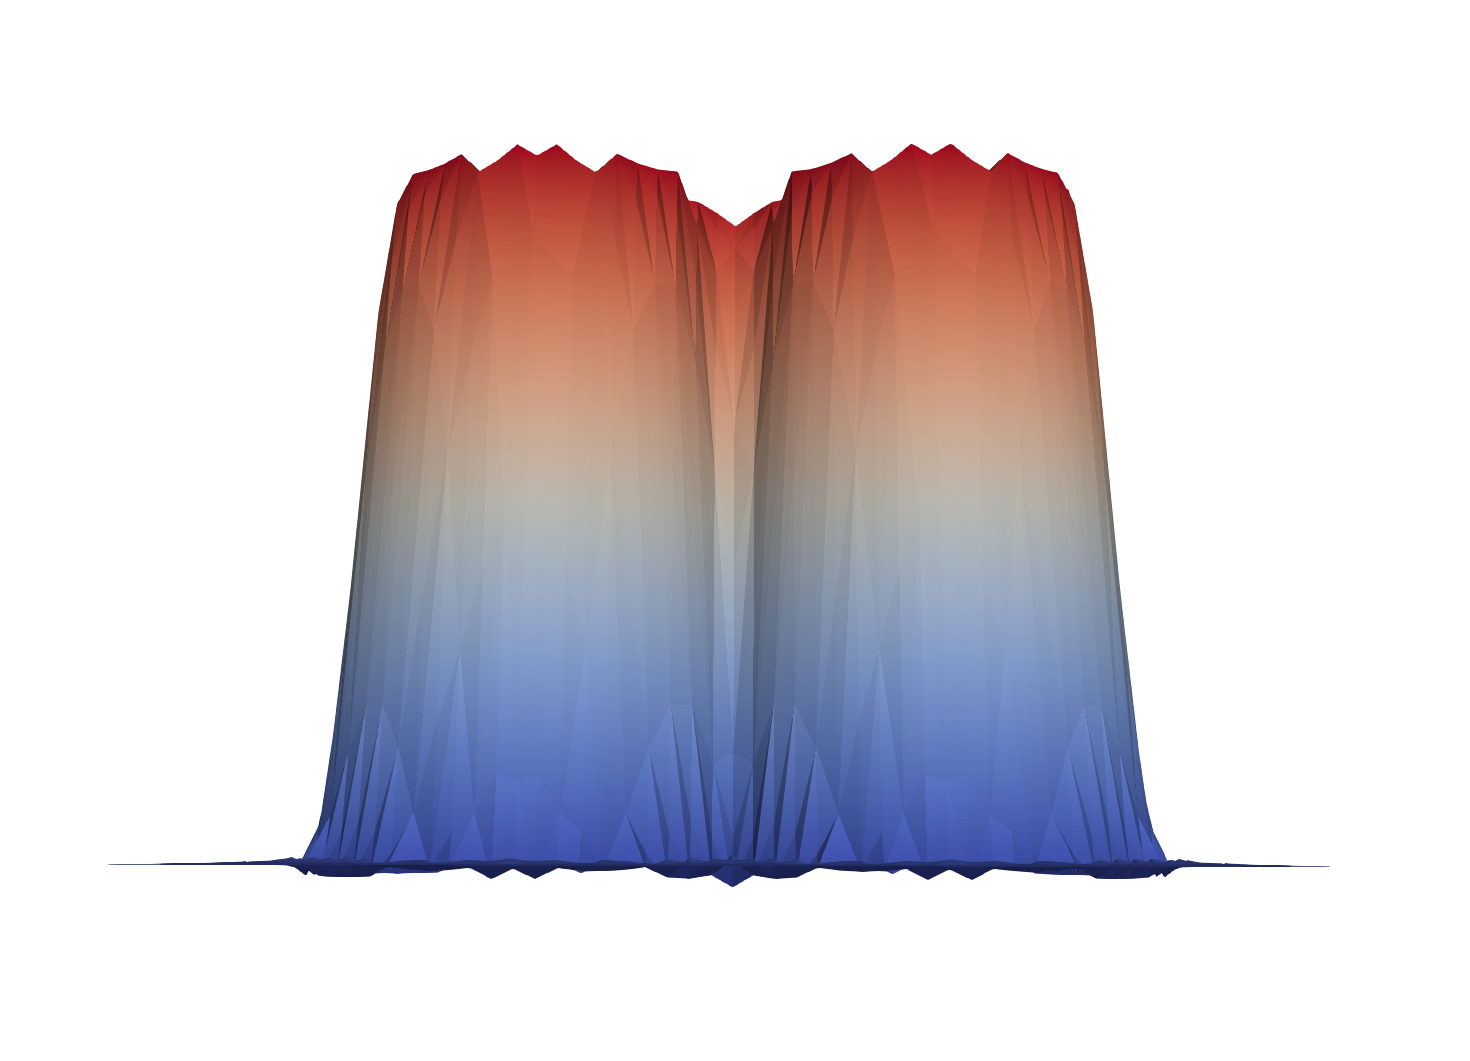
\includegraphics[scale=0.07]{img/non-convective-cahn-hilliard/u_sol_FE_nt-1000_nx-50_T-0.001_P0_adv-0.0_nx-50.png}
		\end{minipage}
		\begin{minipage}{0.32\textwidth}
			\centering
			\textbf{DG-SIP}
			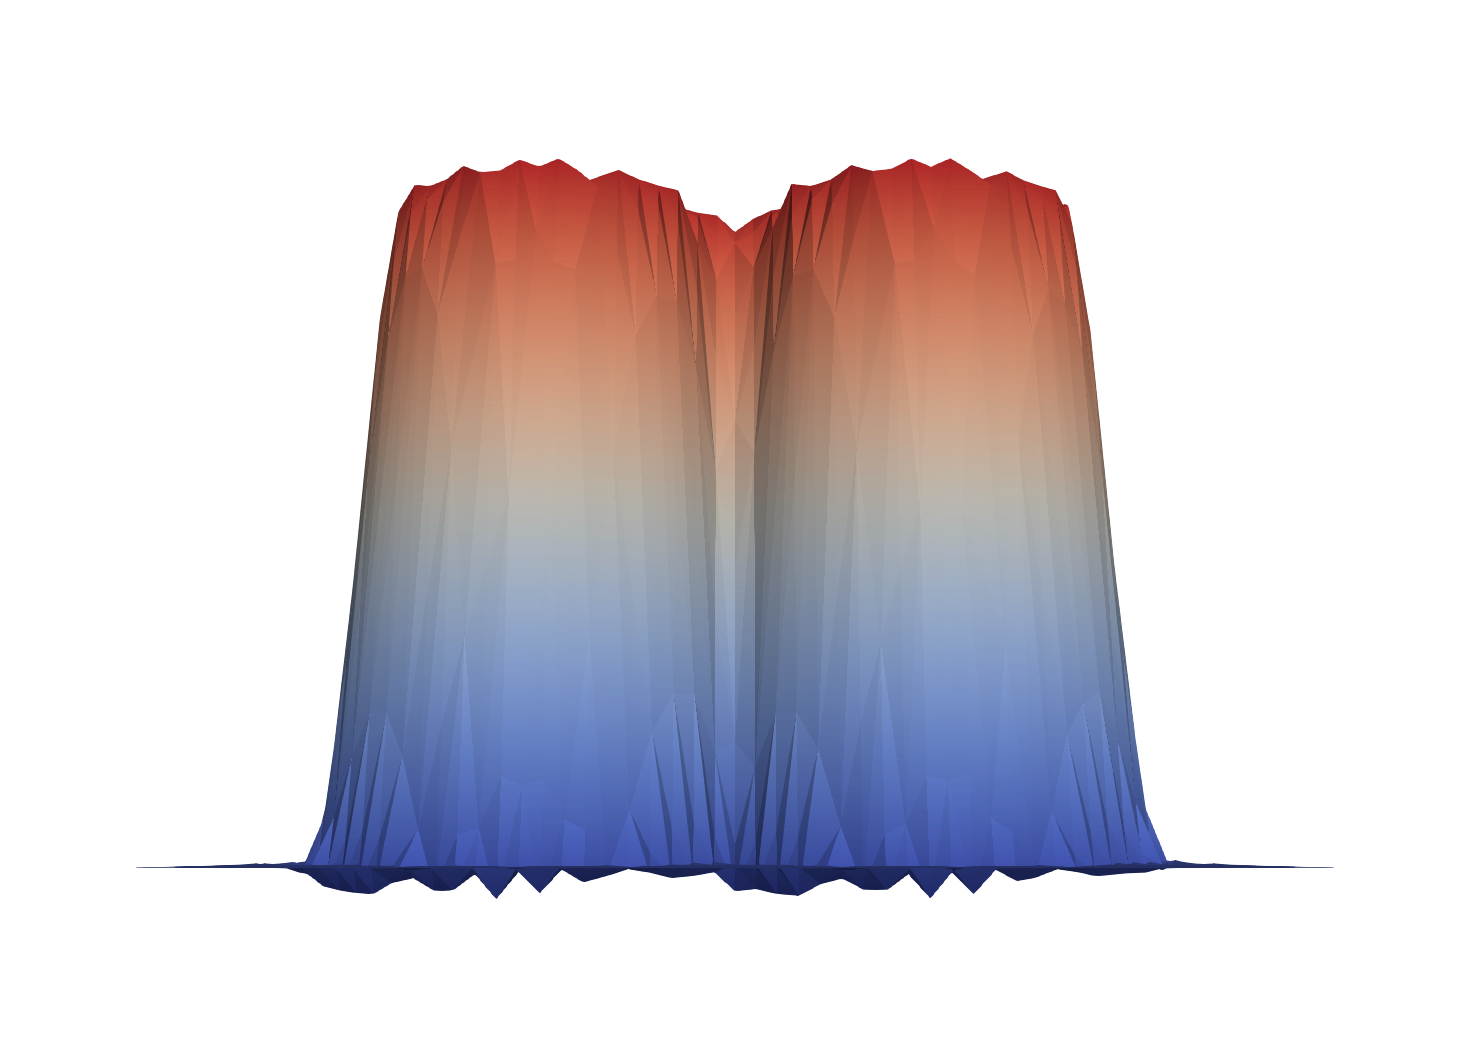
\includegraphics[scale=0.07]{img/non-convective-cahn-hilliard/u_sol_DG-SIP-Sig_nt-1000_nx-50_T-0.001_P0_adv-0.0_nx-50.png}
		\end{minipage}
		\begin{minipage}{0.32\textwidth}
			\centering
			\textbf{DG-UPW}
			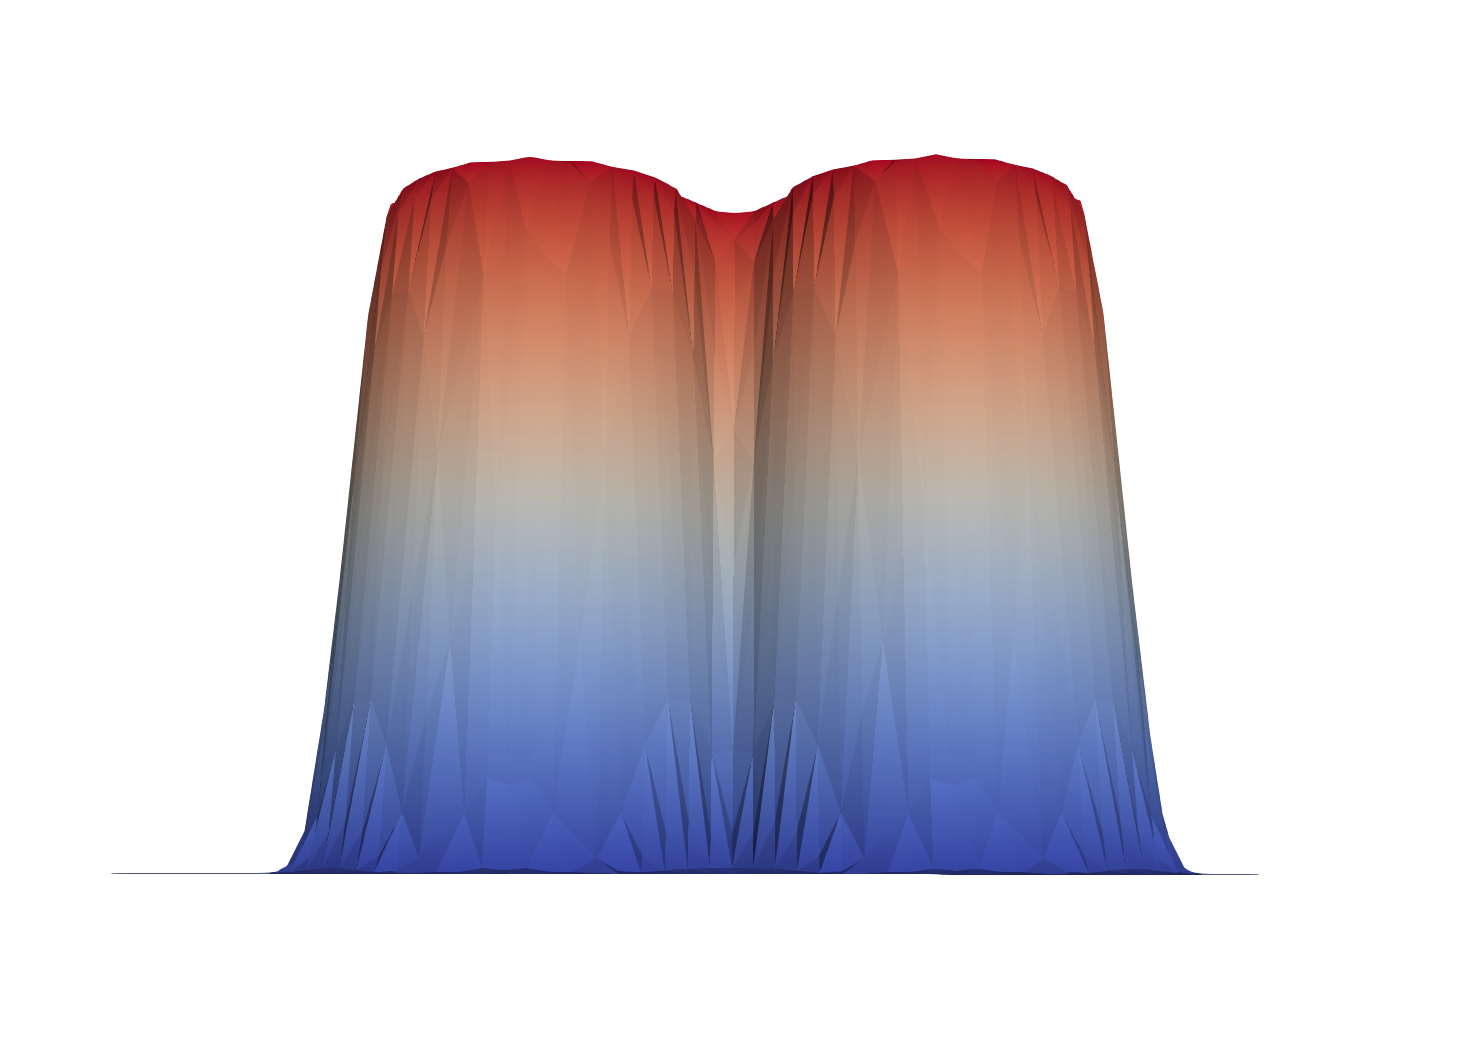
\includegraphics[scale=0.07]{img/non-convective-cahn-hilliard/w_sol_DG-UPW_nt-1000_nx-50_T-0.001_P0_adv-0.0_nx-50.png}
		\end{minipage}
	\end{figure}
\end{frame}

\begin{frame}{Convective Cahn-Hilliard with FEM {\small($\vv=100(y,-x)$)}}
	\vspace{-0.3cm}
	\begin{figure}[t]
		\begin{subfigure}{0.49\textwidth}
			\centering
			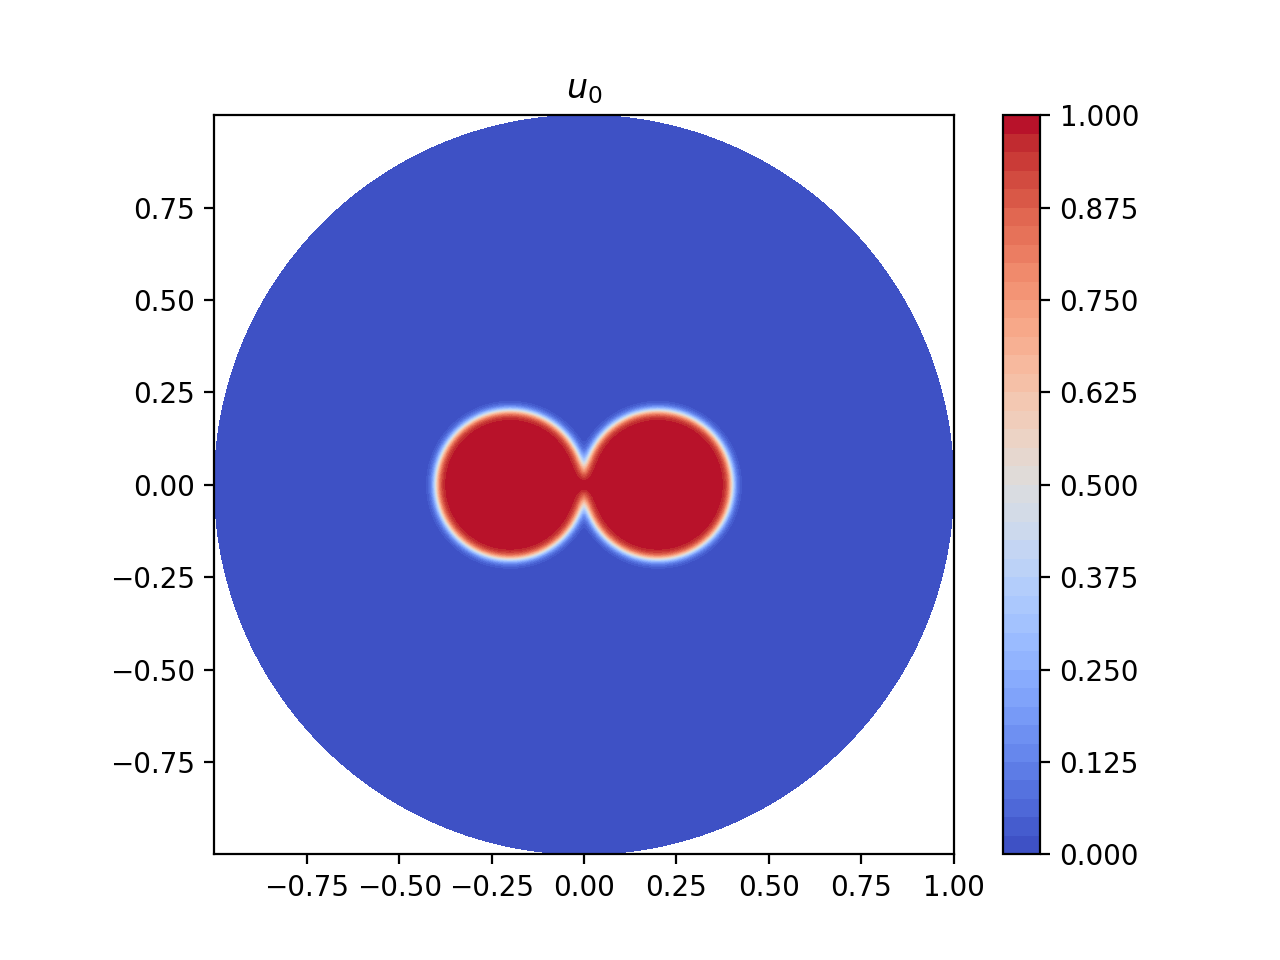
\includegraphics[scale=0.28]{img/convective-cahn-hilliard/u0.png}
		\end{subfigure}
		\hspace*{-1.5cm}
		\begin{subfigure}{0.49\textwidth}
			\centering
			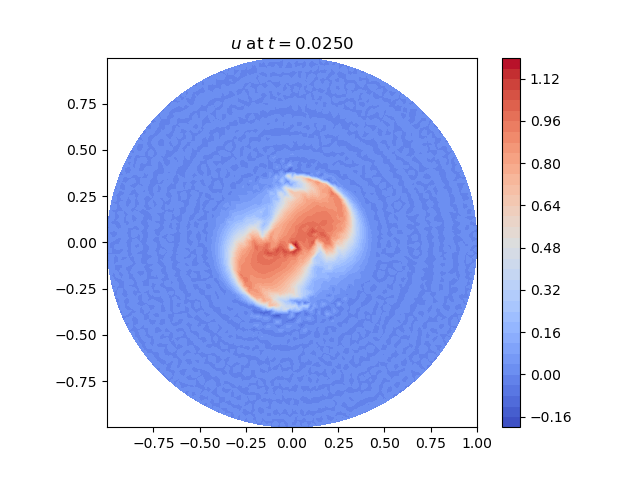
\includegraphics[scale=0.28]{img/convective-cahn-hilliard/u_FE+Eyre_nt-100_t-0.02500_P1_adv-100.0_nx-50.png}
		\end{subfigure}
		\begin{subfigure}{0.49\textwidth}
			\centering
			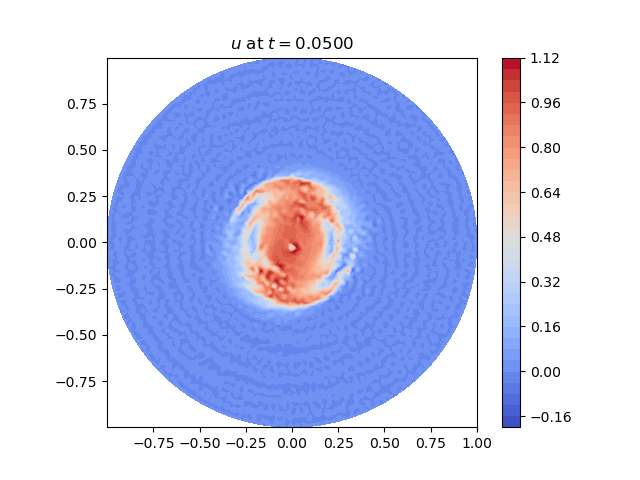
\includegraphics[scale=0.28]{img/convective-cahn-hilliard/u_FE+Eyre_nt-100_t-0.05000_P1_adv-100.0_nx-50.png}
		\end{subfigure}
		\hspace*{-1.5cm}
		\begin{subfigure}{0.49\textwidth}
			\centering
			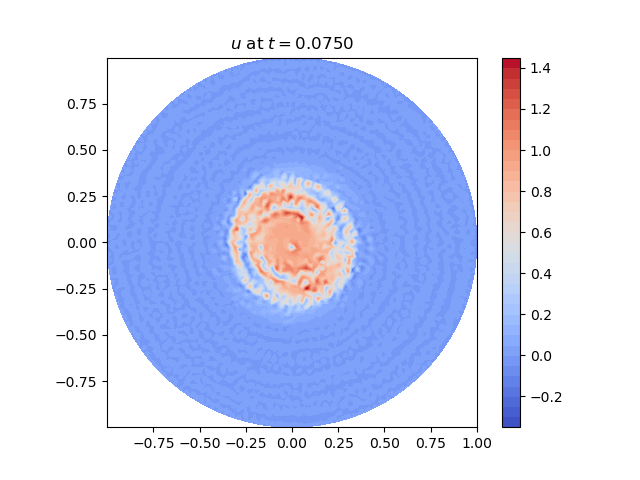
\includegraphics[scale=0.28]{img/convective-cahn-hilliard/u_FE+Eyre_nt-100_t-0.07500_P1_adv-100.0_nx-50.png}
		\end{subfigure}
	\end{figure}
\end{frame}

\begin{frame}{Convective Cahn-Hilliard with DG-SIP {\small($\vv=100(y,-x)$)}}
	\vspace{-0.3cm}
	\begin{figure}[t]
		\begin{subfigure}{0.49\textwidth}
			\centering
			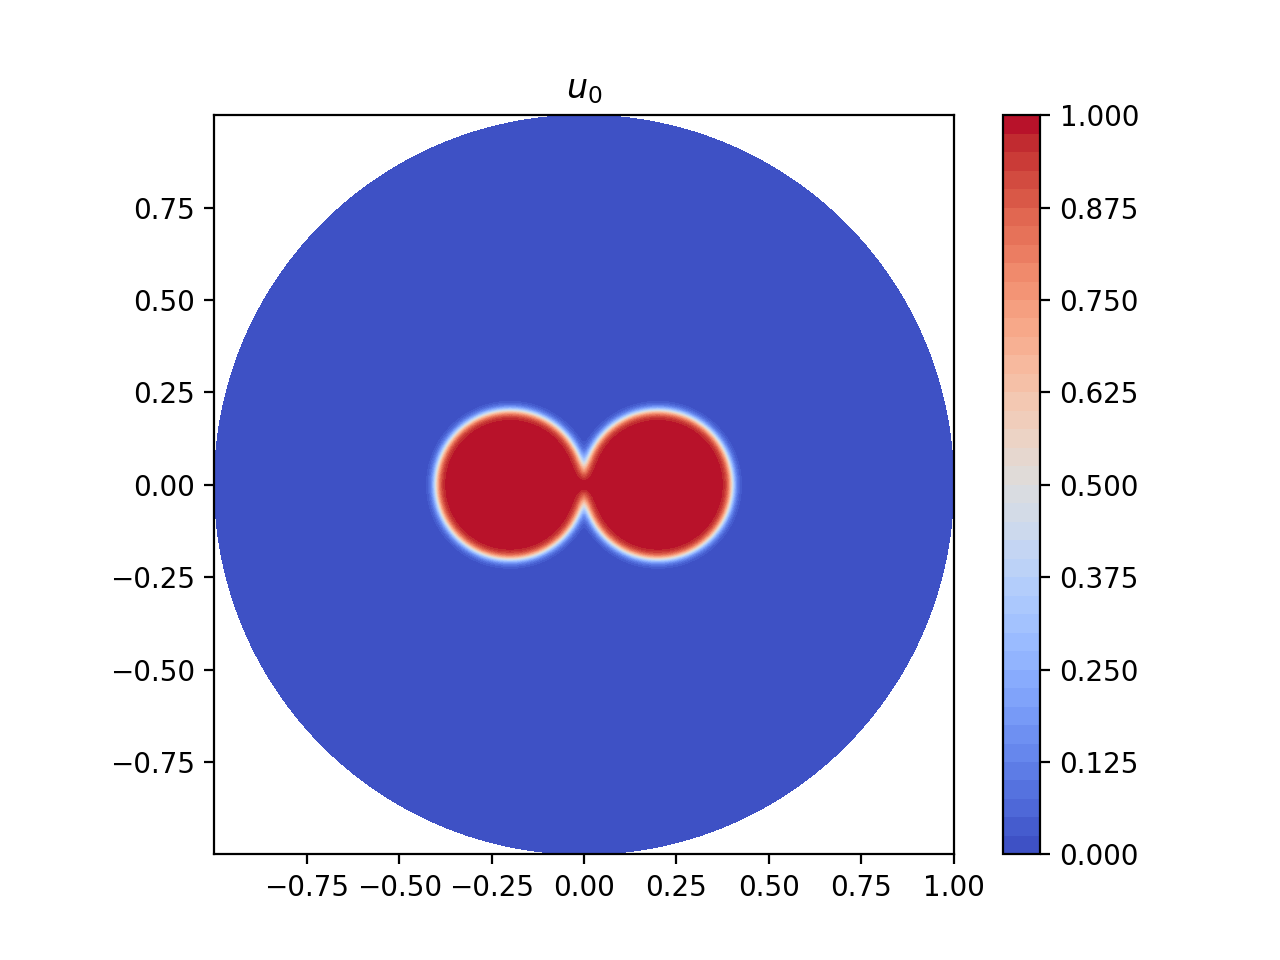
\includegraphics[scale=0.28]{img/convective-cahn-hilliard/u0.png}
		\end{subfigure}
		\hspace*{-1.5cm}
		\begin{subfigure}{0.49\textwidth}
			\centering
			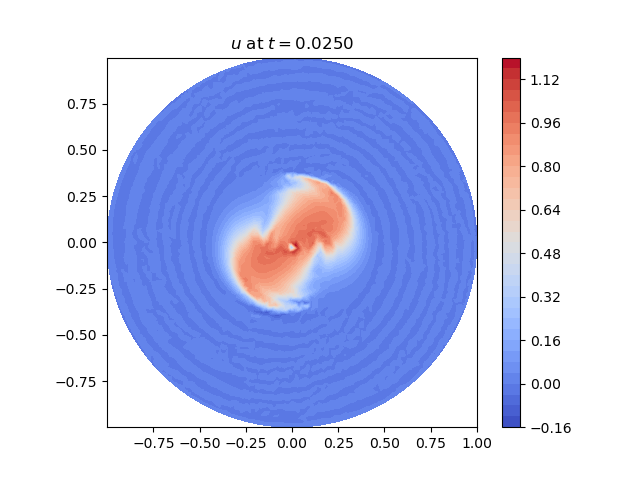
\includegraphics[scale=0.28]{img/convective-cahn-hilliard/u_DG-SIP-Sig+Eyre_nt-100_t-0.02500_P1_adv-100.0_nx-50.png}
		\end{subfigure}
		\begin{subfigure}{0.49\textwidth}
			\centering
			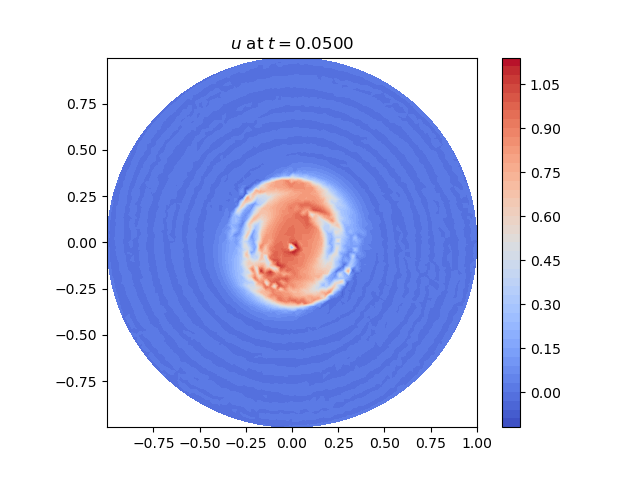
\includegraphics[scale=0.28]{img/convective-cahn-hilliard/u_DG-SIP-Sig+Eyre_nt-100_t-0.05000_P1_adv-100.0_nx-50.png}
		\end{subfigure}
		\hspace*{-1.5cm}
		\begin{subfigure}{0.49\textwidth}
			\centering
			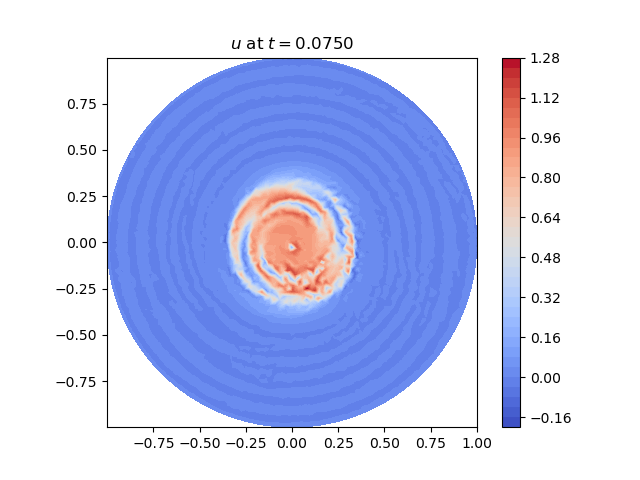
\includegraphics[scale=0.28]{img/convective-cahn-hilliard/u_DG-SIP-Sig+Eyre_nt-100_t-0.07500_P1_adv-100.0_nx-50.png}
		\end{subfigure}
	\end{figure}
\end{frame}

\begin{frame}{Convective Cahn-Hilliard with DG-UPW \small{($\vv=100(y,-x)$)}}
	\vspace{-0.3cm}
	\begin{figure}[t]
		\begin{subfigure}{0.49\textwidth}
			\centering
			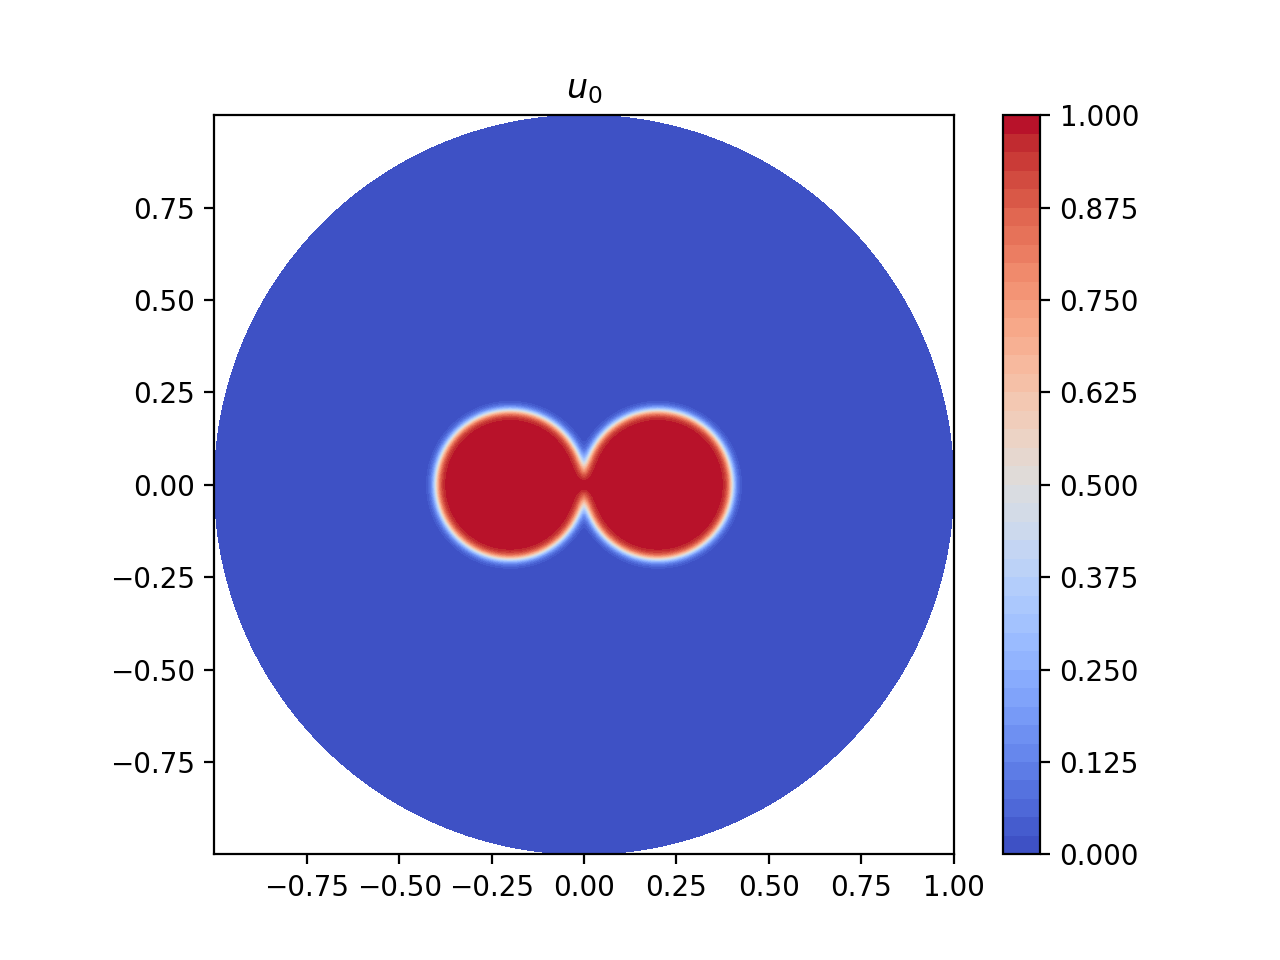
\includegraphics[scale=0.28]{img/convective-cahn-hilliard/u0.png}
		\end{subfigure}
		\hspace*{-1.5cm}
		\begin{subfigure}{0.49\textwidth}
			\centering
			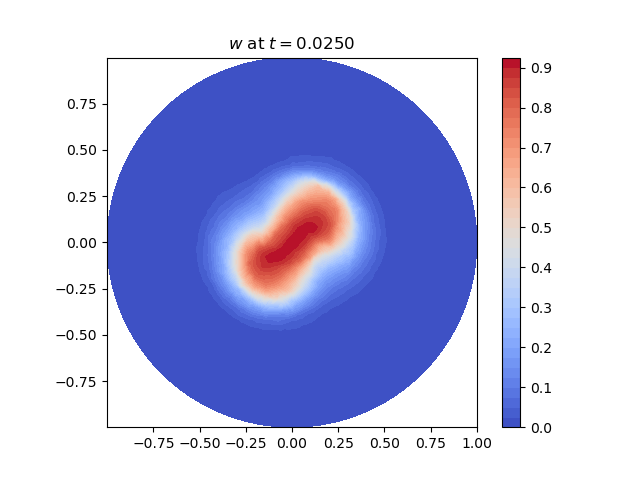
\includegraphics[scale=0.28]{img/convective-cahn-hilliard/w_DG-UPW+Eyre_nt-100_t-0.02500_P0_adv-100.0_nx-50.png}
		\end{subfigure}
		\begin{subfigure}{0.49\textwidth}
			\centering
			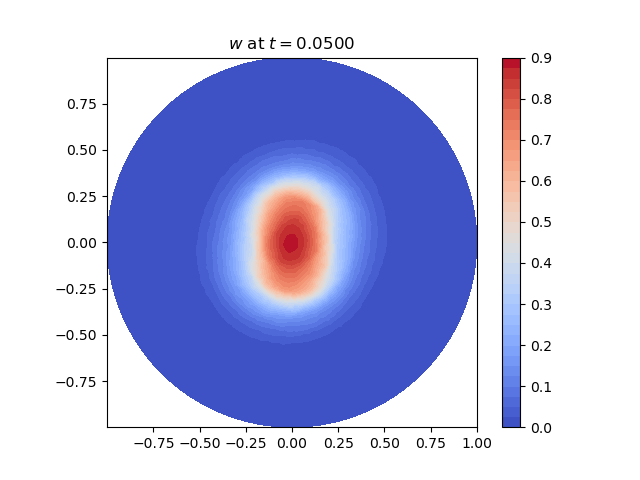
\includegraphics[scale=0.28]{img/convective-cahn-hilliard/w_DG-UPW+Eyre_nt-100_t-0.05000_P0_adv-100.0_nx-50.png}
		\end{subfigure}
		\hspace*{-1.5cm}
		\begin{subfigure}{0.49\textwidth}
			\centering
			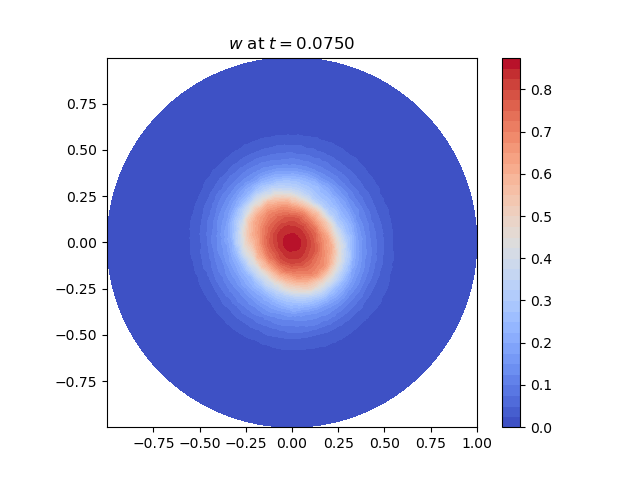
\includegraphics[scale=0.28]{img/convective-cahn-hilliard/w_DG-UPW+Eyre_nt-100_t-0.07500_P0_adv-100.0_nx-50.png}
		\end{subfigure}
	\end{figure}
\end{frame}

\begin{frame}{Convective Cahn-Hilliard \small{($\vv=100(y,-x)$)}}
	\begin{figure}[t]
		\centering
		\begin{minipage}{0.49\linewidth}
			\centering
			\textbf{Maximum-Minimum}\par\smallskip
			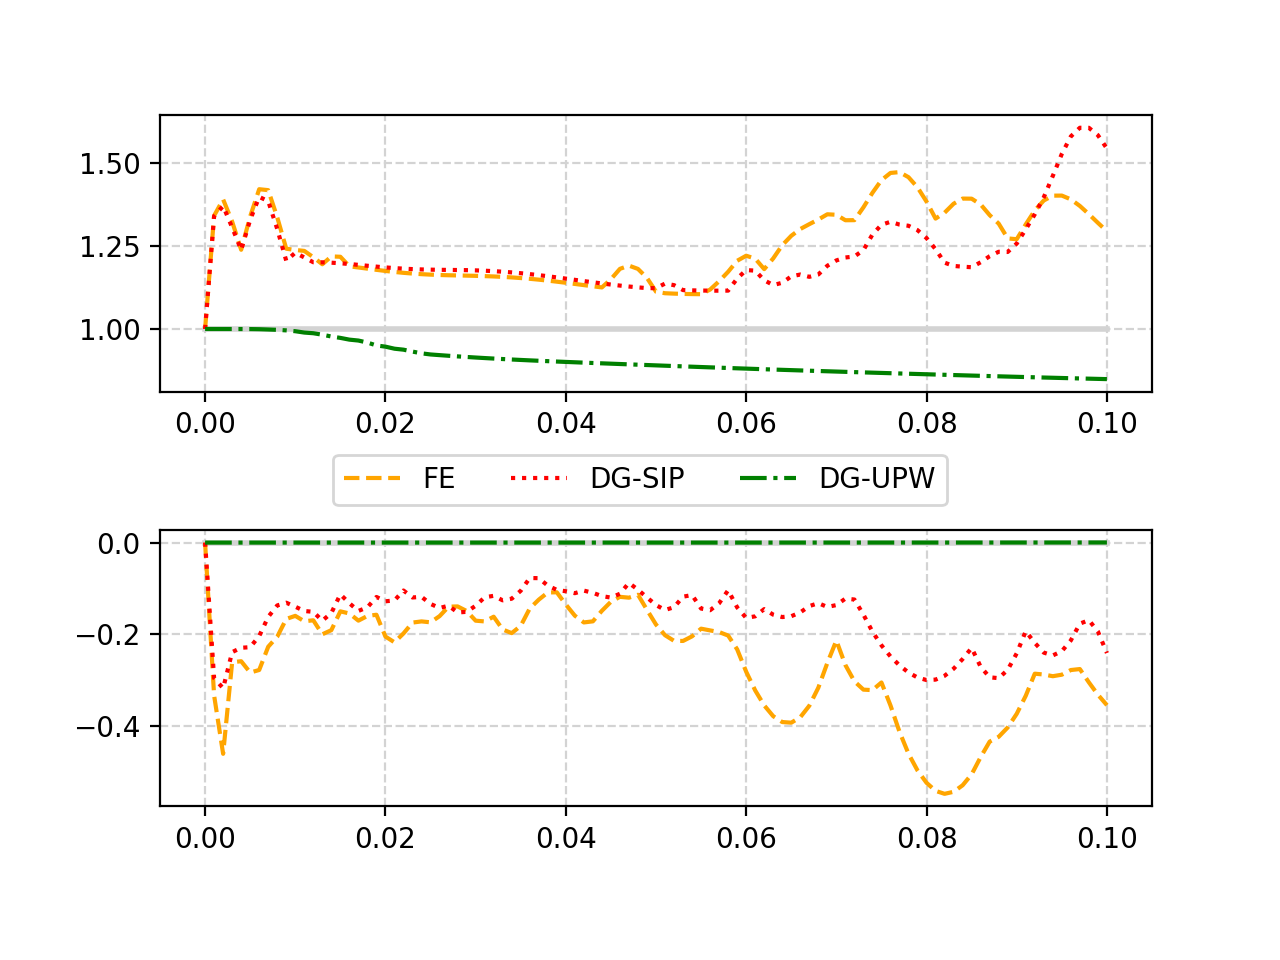
\includegraphics[scale=0.37]{img/convective-cahn-hilliard/max-min_adv-100.png}
		\end{minipage}
		\begin{minipage}{0.49\linewidth}
			\centering
			\textbf{Dynamics}
			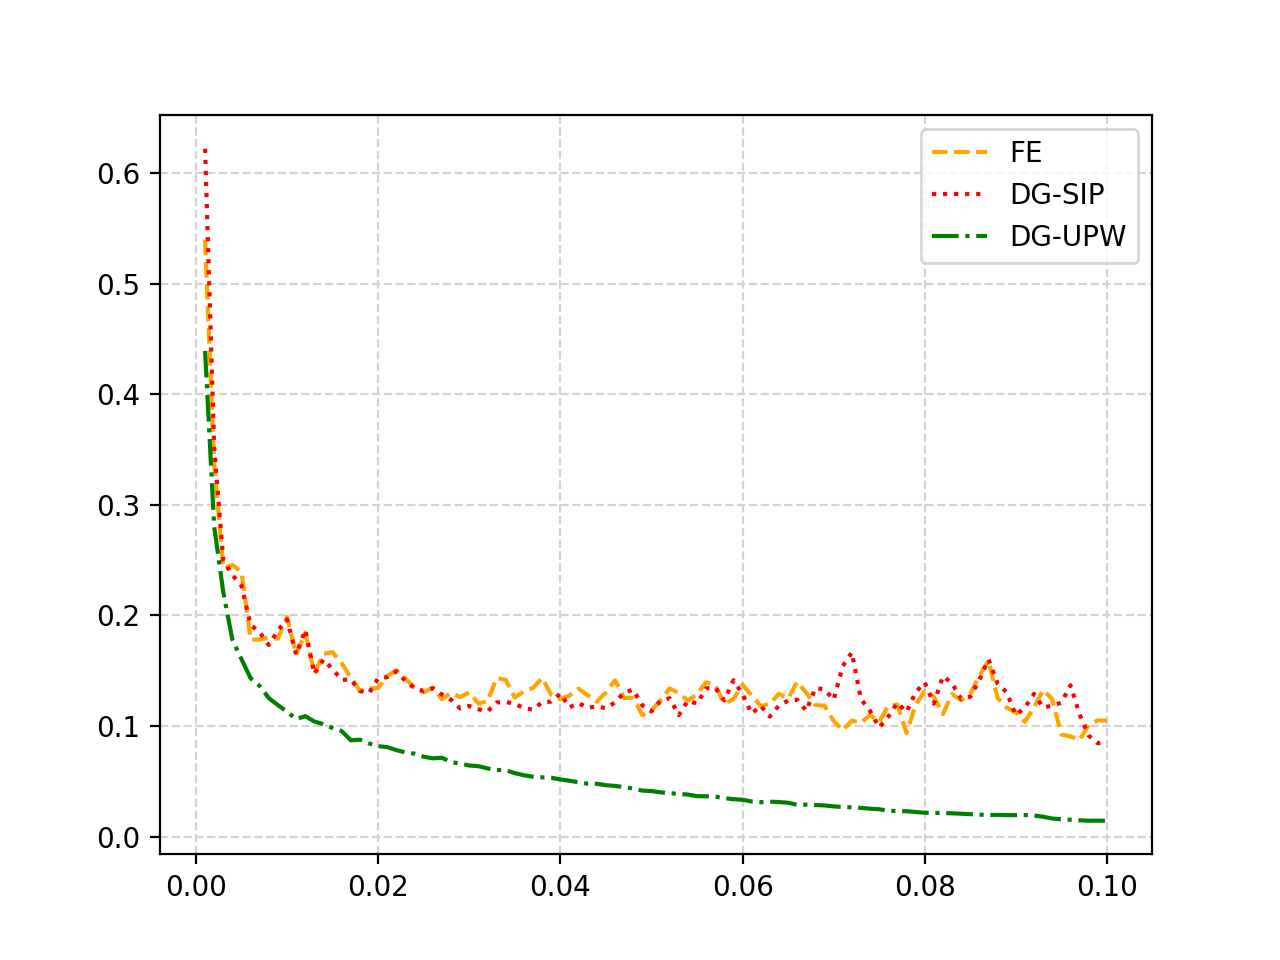
\includegraphics[scale=0.37]{img/convective-cahn-hilliard/dynamics_adv-100.png}
		\end{minipage}
		\caption{On the left, maximum and minimum of the phase field variable over time. On the right, we plot $\frac{\normaLinf{u^{m+1}-u^m}}{\normaLinf{u^m}}$ to observe the dynamics of the approximations.}
	\end{figure}
\end{frame}

\begin{frame}{Stokes-Cahn-Hilliard with FEM {\small(cavity test)}}
	\vspace{-0.3cm}
	\begin{figure}[t]
		\begin{subfigure}{0.49\textwidth}
			\centering
			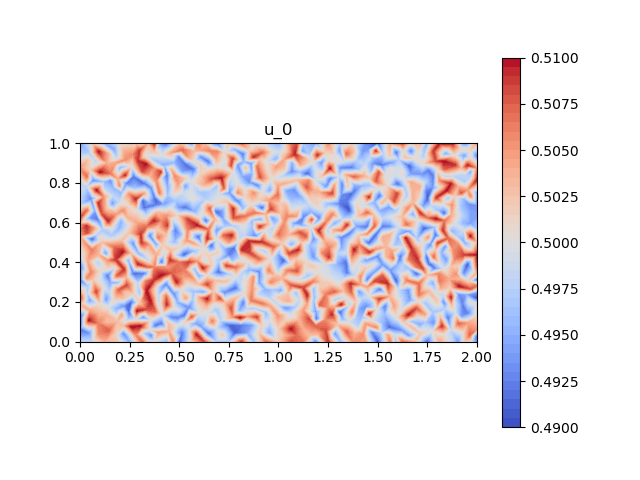
\includegraphics[scale=0.28]{img/stokes-cahn-hilliard/u_stokes_initial_condition.png}
		\end{subfigure}
		\hspace*{-1.5cm}
		\begin{subfigure}{0.49\textwidth}
			\centering
			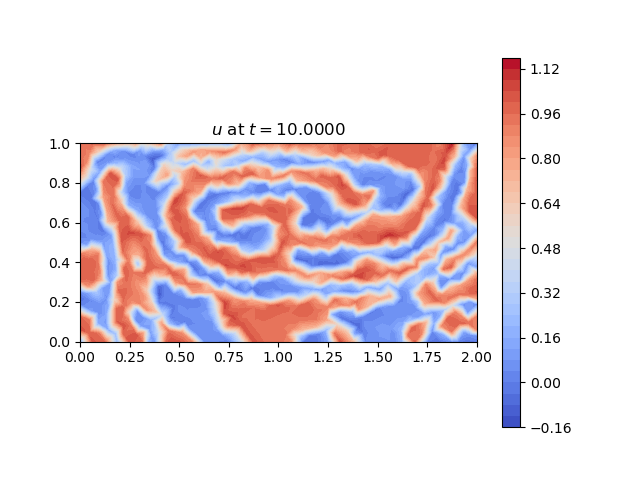
\includegraphics[scale=0.28]{img/stokes-cahn-hilliard/u_FE+Eyre_stokes_nt-40000_t-10.00000_P1.png}
		\end{subfigure}
		\begin{subfigure}{0.49\textwidth}
			\centering
			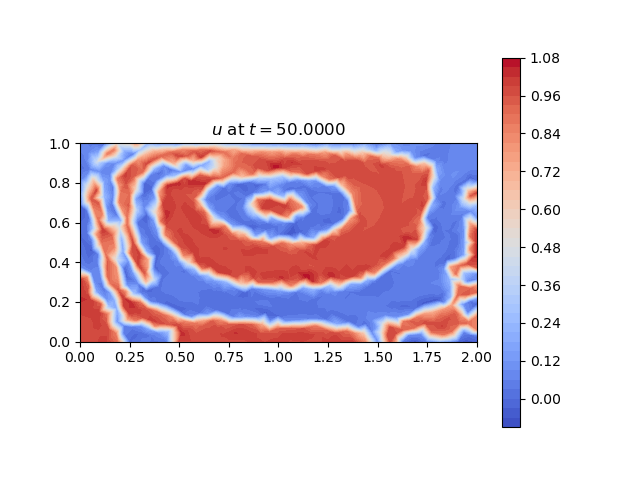
\includegraphics[scale=0.28]{img/stokes-cahn-hilliard/u_FE+Eyre_stokes_nt-40000_t-50.00000_P1.png}
		\end{subfigure}
		\hspace*{-1.5cm}
		\begin{subfigure}{0.49\textwidth}
			\centering
			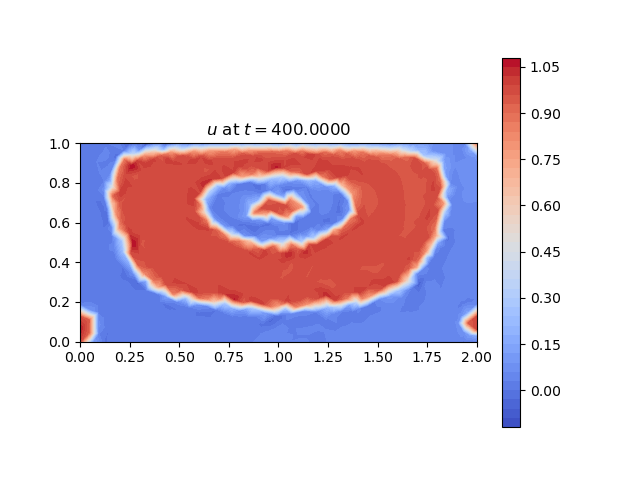
\includegraphics[scale=0.28]{img/stokes-cahn-hilliard/u_FE+Eyre_stokes_nt-40000_t-400.00000_P1.png}
		\end{subfigure}
	\end{figure}
\end{frame}

\begin{frame}{Stokes-Cahn-Hilliard with DG-SIP {\small(cavity test)}}
	\vspace{-0.3cm}
	\begin{figure}[t]
		\begin{subfigure}{0.49\textwidth}
			\centering
			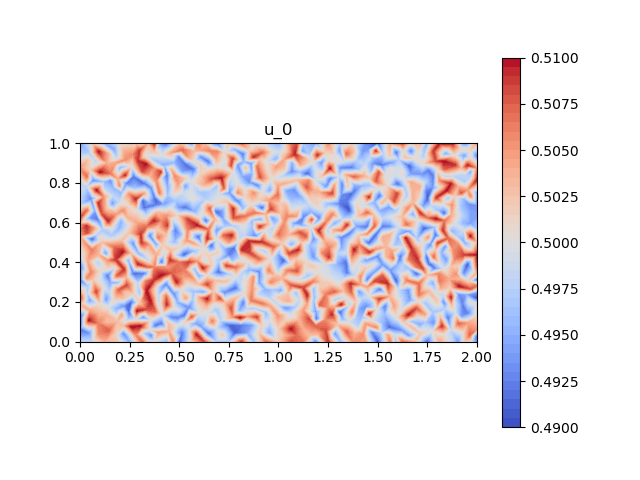
\includegraphics[scale=0.28]{img/stokes-cahn-hilliard/u_stokes_initial_condition.png}
		\end{subfigure}
		\hspace*{-1.5cm}
		\begin{subfigure}{0.49\textwidth}
			\centering
			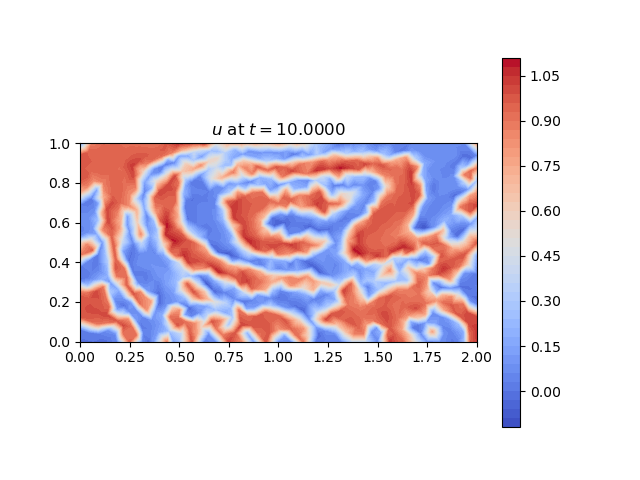
\includegraphics[scale=0.28]{img/stokes-cahn-hilliard/u_DG-SIP-Sig+Eyre_stokes_nt-40000_t-10.00000_P1.png}
		\end{subfigure}
		\begin{subfigure}{0.49\textwidth}
			\centering
			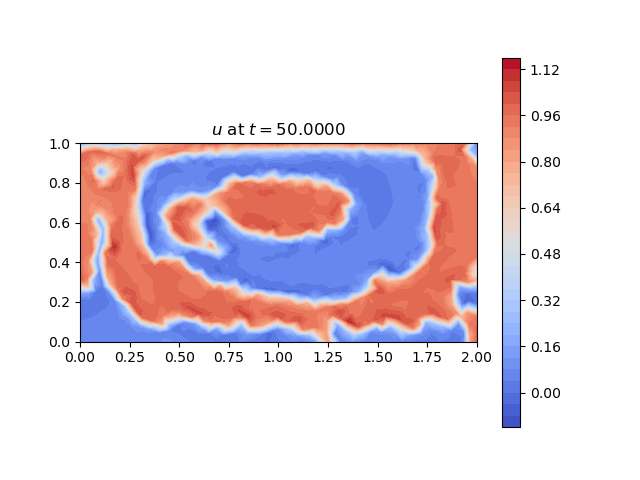
\includegraphics[scale=0.28]{img/stokes-cahn-hilliard/u_DG-SIP-Sig+Eyre_stokes_nt-40000_t-50.00000_P1.png}
		\end{subfigure}
		\hspace*{-1.5cm}
		\begin{subfigure}{0.49\textwidth}
			\centering
			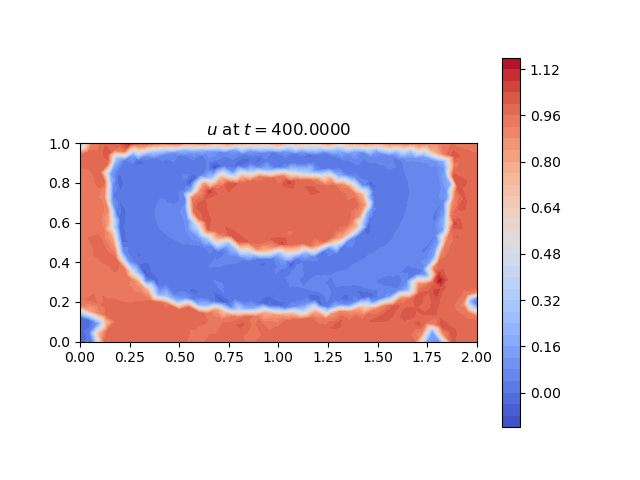
\includegraphics[scale=0.28]{img/stokes-cahn-hilliard/u_DG-SIP-Sig+Eyre_stokes_nt-40000_t-400.00000_P1.png}
		\end{subfigure}
	\end{figure}
\end{frame}

\begin{frame}{Stokes-Cahn-Hilliard with DG-UPW {\small(cavity test)}}
	\vspace{-0.3cm}
	\begin{figure}[t]
		\begin{subfigure}{0.49\textwidth}
			\centering
			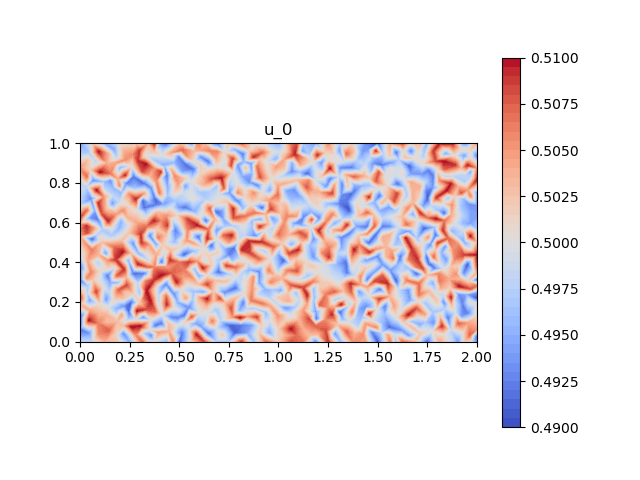
\includegraphics[scale=0.28]{img/stokes-cahn-hilliard/u_stokes_initial_condition.png}
		\end{subfigure}
		\hspace*{-1.5cm}
		\begin{subfigure}{0.49\textwidth}
			\centering
			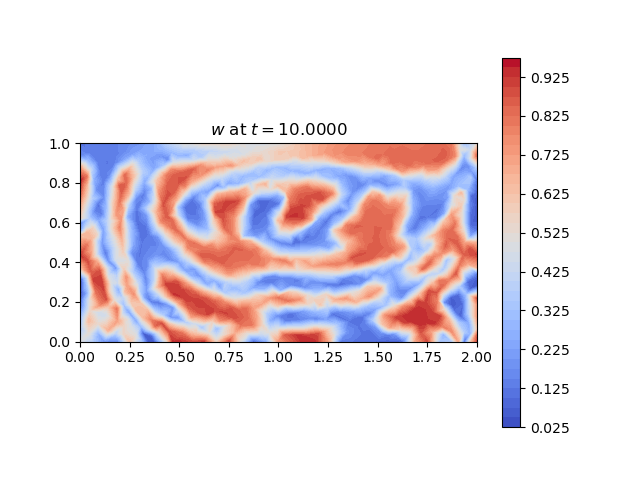
\includegraphics[scale=0.28]{img/stokes-cahn-hilliard/w_DG-UPW+Eyre_stokes_nt-40000_t-10.00000_P0.png}
		\end{subfigure}
		\begin{subfigure}{0.49\textwidth}
			\centering
			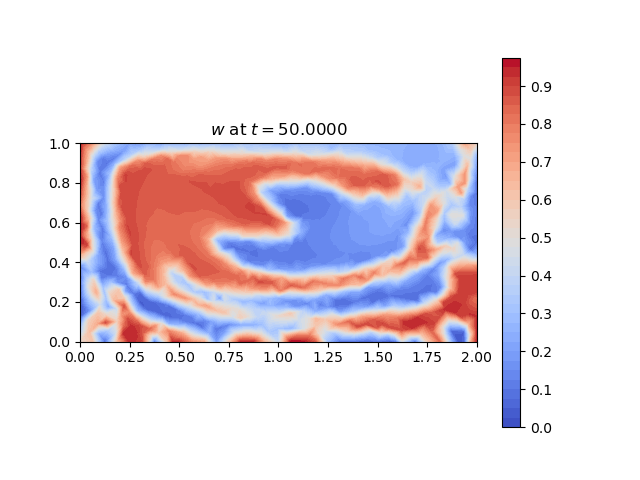
\includegraphics[scale=0.28]{img/stokes-cahn-hilliard/w_DG-UPW+Eyre_stokes_nt-40000_t-50.00000_P0.png}
		\end{subfigure}
		\hspace*{-1.5cm}
		\begin{subfigure}{0.49\textwidth}
			\centering
			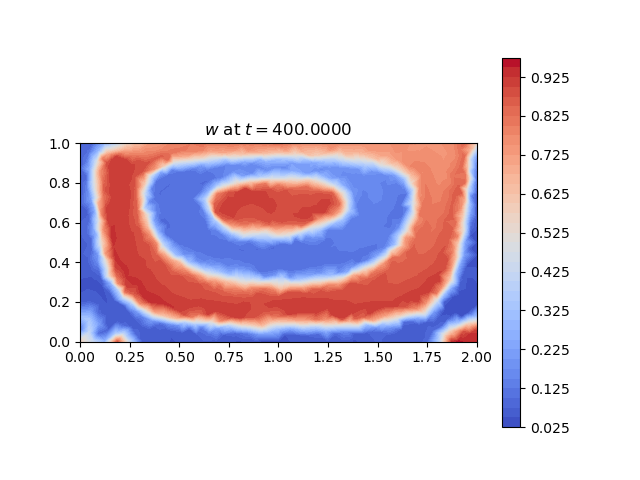
\includegraphics[scale=0.28]{img/stokes-cahn-hilliard/w_DG-UPW+Eyre_stokes_nt-40000_t-400.00000_P0.png}
		\end{subfigure}
	\end{figure}
\end{frame}

\begin{frame}{Stokes-Cahn-Hilliard {\small(cavity test)}}
	\begin{figure}[t]
		\centering
		\begin{minipage}{0.49\linewidth}
			\centering
			\textbf{Maximum-Minimum}\par\smallskip
			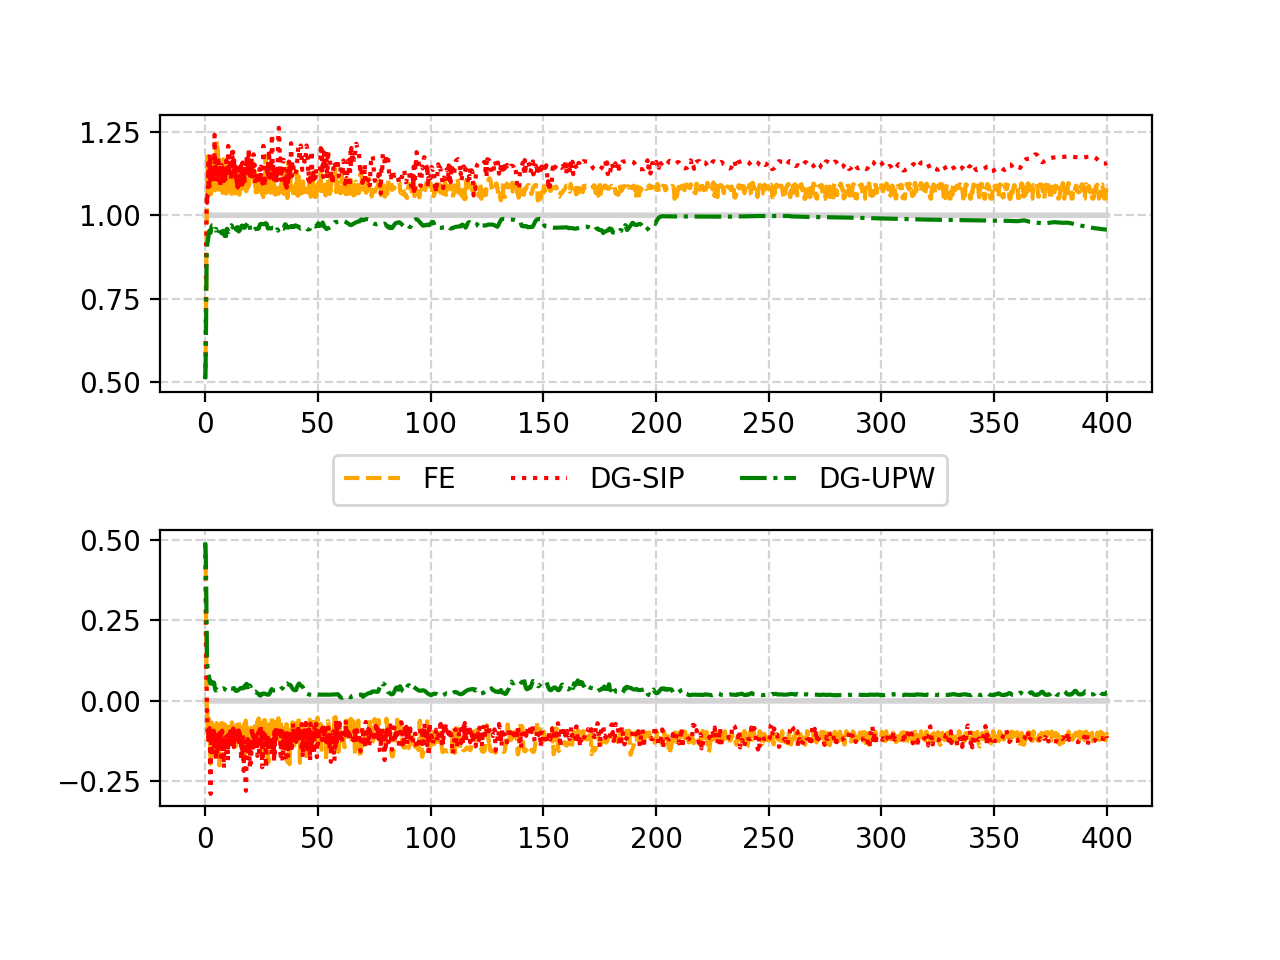
\includegraphics[scale=0.37]{img/stokes-cahn-hilliard/max-min_stokes.png}
		\end{minipage}
		\begin{minipage}{0.49\linewidth}
			\centering
			\textbf{Dynamics}
			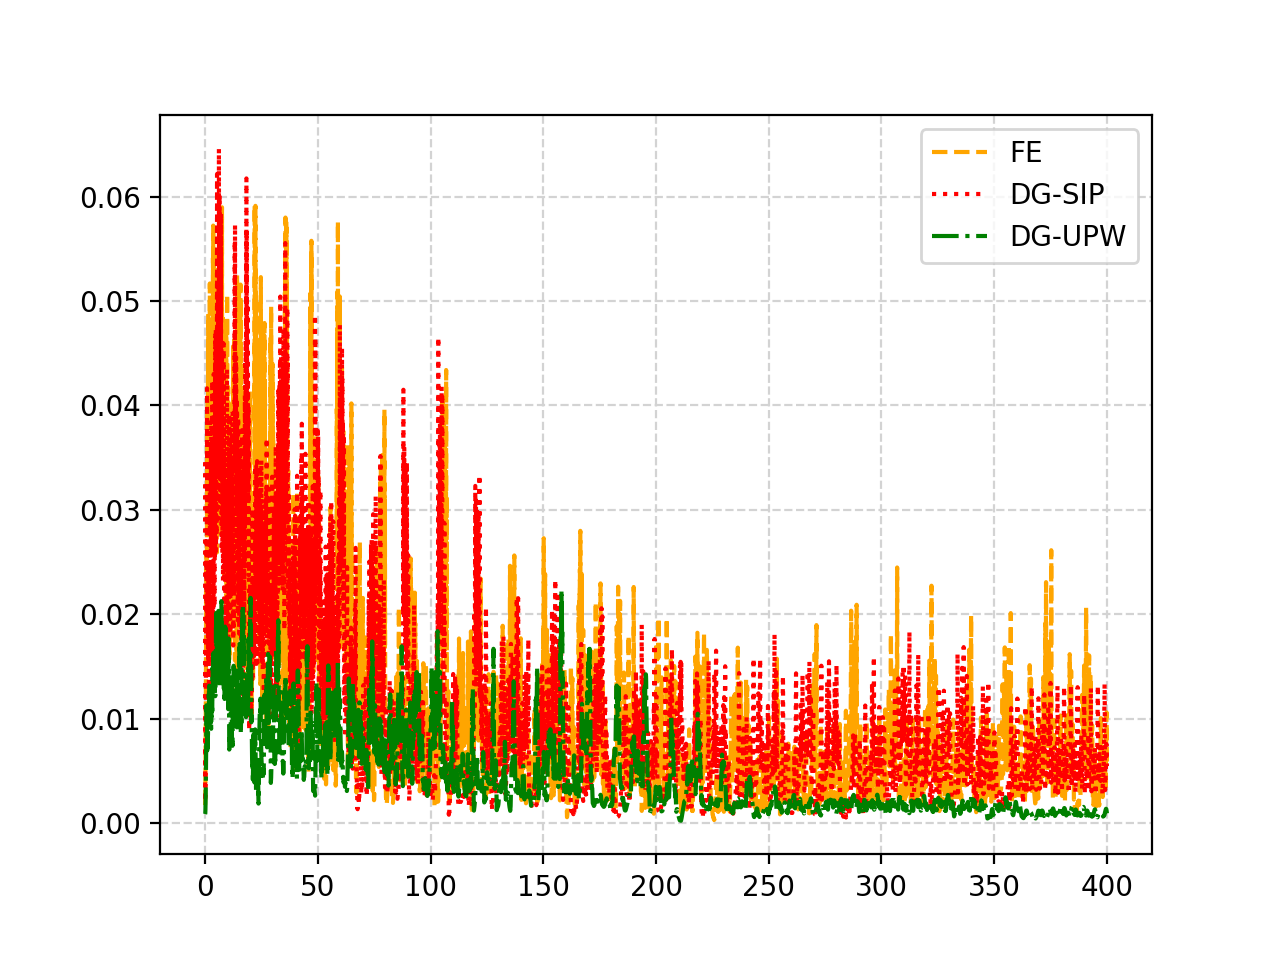
\includegraphics[scale=0.37]{img/stokes-cahn-hilliard/dynamics_stokes.png}
		\end{minipage}
		\caption{On the left, maximum and minimum of the phase field variable over time. On the right, we plot $\frac{\normaLinf{u^{m+1}-u^m}}{\normaLinf{u^m}}$ to observe the dynamics of the approximations.}
	\end{figure}
\end{frame}

\begin{frame}{Convergence order: non-convective Cahn-Hilliard}
	\begin{table}
		%%% TABLE WITH T=0.001 %%%
		\begin{center}
				\fontsize{4pt}{6pt}\selectfont
				{\footnotesize\structure{Table:} Errors and convergence orders at $T=0.001$ without convection ($\vv=0$).\vspace*{0.3cm} }
				\begin{tabular}{ccccccccc}
					\toprule
					\multirow{2}[2]{*}{Scheme} & \multirow{2}[2]{*}{Norm}& $h\approx 2.8284\cdot 10^{-2}$ & \multicolumn{2}{c}{$h/2\approx 1.4142\cdot 10^{-2}$} & \multicolumn{2}{c}{$h/3\approx 9.428\cdot 10^{-3}$} &\multicolumn{2}{c}{$h/4\approx 7.071\cdot 10^{-3}$} \\
					\cline{3-9}
					&&Error &Error & Order &  Error & Order &  Error & Order \\
					\midrule
					\multirow{2}[2]{*}{\textbf{DG-UPW}} & $\norma{\cdot}_{L^2}$ & $8.5268\cdot 10^{-3}$ &$3.0933\cdot 10^{-3}$ & $1.46$ &$1.7645\cdot 10^{-3}$  & $1.38$  &$1.2134\cdot 10^{-3}$ & $1.30$   \\
					\cline{2-9}
					& $\norma{\cdot}_{H^1}$ &$8.0000\cdot 10^{-1}$  &$4.0199\cdot 10^{-1}$  & $0.99$ &$2.6081\cdot 10^{-1}$ & $1.07$  &$1.8849\cdot 10^{-1}$ & $1.13$   \\
					\midrule
					\multirow{2}[2]{*}{FEM}  & $\norma{\cdot}_{L^2}$ &$5.3224\cdot 10^{-3}$  &$1.5679\cdot 10^{-3}$ &$1.76$ &$6.9944\cdot 10^{-4}$  &$1.99$ &$4.0191\cdot 10^{-4}$ & $1.93$ \\
					\cline{2-9}
					& $\norma{\cdot}_{H^1}$ &$8.9963\cdot 10^{-1}$  & $4.1080\cdot 10^{-1}$ & $1.13$  &$2.5252\cdot 10^{-1}$  & $1.2$   &$1.7799\cdot 10^{-1}$  & $1.22$  \\
					\midrule
					\multirow{2}[2]{*}{DG-SIP}  & $\norma{\cdot}_{L^2}$ &$4.6466\cdot 10^{-3}$  &$1.3023\cdot 10^{-3}$  & $1.84$  &$5.8945\cdot 10^{-4}$ & $1.96$ &$3.2710\cdot 10^{-4}$ & $2.05$   \\
					\cline{2-9}
					& $\norma{\cdot}_{H^1}$ &$1.1784$  &$5.8331\cdot 10^{-1}$  & $1.01$  &$3.6254\cdot 10^{-1}$ & $1.17$  &$2.6024\cdot 10^{-1}$ &$1.15$ \\
					\bottomrule
				\end{tabular}
		\end{center}
	\end{table}
\end{frame}

\begin{frame}{Convergence order: convective Cahn-Hilliard }
	\begin{table}
		%%% TABLE WITH T=0.001 %%%
		\begin{center}
				\fontsize{4pt}{6pt}\selectfont
				{\footnotesize\structure{Table:} Errors and convergence orders at $T=0.001$ with convection ($\vv=(y,-x)$).\vspace*{0.3cm}}
				\begin{tabular}{ccccccccc}
					\toprule
					\multirow{2}[2]{*}{Scheme} & \multirow{2}[2]{*}{Norm}& $h\approx 4\cdot 10^{-2}$ & \multicolumn{2}{c}{$h/2\approx 2\cdot 10^{-2} $} & \multicolumn{2}{c}{$h/3\approx 1.3333\cdot 10^{-2}$} &\multicolumn{2}{c}{$h/4\approx 1\cdot 10^{-2}$} \\
					\cline{3-9}
					&&Error &Error & Order &  Error & Order &  Error & Order \\
					\midrule
					\multirow{2}[2]{*}{\textbf{DG-UPW}} & $\norma{\cdot}_{L^2}$ &$1.7288\cdot 10^{-2}$  &$6.9446\cdot 10^{-3}$ & $1.32$  &$3.3102\cdot 10^{-3}$ & $1.83$  &$2.0578\cdot 10^{-3}$ & $1.65$   \\
					\cline{2-9}
					& $\norma{\cdot}_{H^1}$ &$1.4549$ &$6.0305\cdot 10^{-1}$ & $1.27$ &$3.0204\cdot 10^{-1}$ & $1.71$ &$2.0315\cdot 10^{-1}$ & $1.38$  \\
					\midrule
					\multirow{2}[2]{*}{FEM}  & $\norma{\cdot}_{L^2}$ &$6.8347\cdot 10^{-3}$  &$2.1213\cdot 10^{-3}$  & $1.69$  &$9.7749\cdot 10^{-4}$ & $1.91$  &$5.3883\cdot 10^{-4}$ & $2.07$ \\
					\cline{2-9}
					& $\norma{\cdot}_{H^1}$ &$8.3104\cdot 10^{-1}$  &$3.8060\cdot 10^{-1}$  & $1.13$  &$2.1887\cdot 10^{-1}$ & $1.36$ &$1.4991\cdot 10^{-1}$ & $1.32$  \\
					\midrule
					\multirow{2}[2]{*}{DG-SIP}  & $\norma{\cdot}_{L^2}$ &$6.5242\cdot 10^{-3}$  & $1.9557\cdot 10^{-3}$  & $1.74$ &$8.9471\cdot 10^{-4}$  & $1.93$ &$5.0257\cdot 10^{-4}$ & $2.00$ \\
					\cline{2-9}
					& $\norma{\cdot}_{H^1}$ &$1.1980$ &$6.1624\cdot 10^{-1}$  & $0.96$ &$3.8451\cdot 10^{-1}$  & $1.16$ &$2.7439\cdot 10^{-1}$ &$1.17$ \\
					\bottomrule
				\end{tabular}
		\end{center}
	\end{table}
\end{frame}

\begin{frame}{References}
	\scriptsize 
	\vspace*{-0.25cm}
	\nocite*
	\bibliographystyle{apalike}
	\bibliography{references}
\end{frame}

\begin{frame}{}
	\centering
	\vspace*{1cm}
	{\Huge
		\emph{Thanks for your attention!}}
	
	\vspace*{1cm}
	\begin{acknowledgements}
		The speaker has been supported by a \textit{Graduate Scholarship funded by the University of Tennessee at Chattanooga} and by \textit{UCA FPU contract UCA/REC14VPCT/2020 funded by Universidad de Cádiz}.
		
		The collaborators have been supported by \textit{Grant PGC2018-098308-B-I00} by \textit{MCI N/AEI/ 10.13039/501100011033} and by \textit{ERDF a way of making Europe}.
	\end{acknowledgements}
\end{frame}